\chapter{Ответы на вопросы}


\hspace{0cm} \textbf{1. Укажите интервалы значений аргумента, в которых можно считать решением заданного уравнения каждое из первых 4-х приближений Пикара. Точность результата оценивать до второй цифры после запятой. Объяснить свой ответ.}

Приближение можно считать решением пока его значение совпадает со значением следующего приближения (мы рассматриваем до второй запятой), когда их значения начнут расходиться, нужно рассматривать следующее приближение.

\eq{|y_n(x) - y_{n+1}(x)| < \epsilon,}

Результат:
\begin{itemize}
    \item Для Пикара 1 порядка: (0, 0,937)
    \item Для Пикара 2 порядка: (0, 1,233)
    \item Для Пикара 3 порядка: (0, 1,419)
\end{itemize}

\newpage

\begin{lstlisting}[caption=вычисление крайнего значения аргумента, label=lst1]
    double h = 0.001;  
    double eps = 0.01; 
    double x0 = 0;
    int n = 3;

    while (Math.Abs(Methods.Pikar(x0, n + 1) - Methods.Pikar(x0, n)) < eps)
        {
            x0 += h;
        }
    Console.WriteLine("{0,6:F8}", x0);
\end{lstlisting}

На листинге \ref{lst1} код программы, результат которого является крайнее правое значение аргумента для метода Пикара порядка точности n \\

\hspace{0cm} \textbf{2.  Пояснить, каким образом можно доказать правильность полученного результата при фиксированном значении аргумента в численных методах.}

При фиксированном значении аргумента надо менять шаг и наблюдать, как ведёт себя решение. Если наступает такой момент с уменьшением шага, когда функция перестаёт меняться, это и есть истинное решение. Ибо сходимость определяется при фиксированном значении аргумента, как разность между точным значением и приближённым. По мере того, как шаг уменьшается, точность возрастает. \\

\hspace{0cm} \textbf{3. Каково значение функции при $x=2$, т.е. привести значение $u(2)$.}

По схеме ответа на вопрос №2 рассчитаем значение $u(2)$

\begin{lstlisting}[caption=вычисление значение функции при $u(2)$, label=lst2]
    double x0 = 0;
    double y = 0;
    double h = 0.1;
    double xMax = 2;
    int i = 0;
    Console.WriteLine("|     h    |    x     |");
    while (i < 8)
        {
            y = 0;
            x0 = 0;
            while (x0 < xMax)
                {
                    y = Methods.EulerOpened(x0, h, y);
                    x0 += h;
                }

            Console.WriteLine("|{0,6:F8}|{1,6:F8}|", h, y);
            h *= 0.1;
            i++;
        }
\end{lstlisting}

На листинге \ref{lst2} показан код, который находит значение $u(2)$, а на рисунке \ref{fig:fig1}, показан вывод программы.

\begin{figure}[ht!]
  \centering
  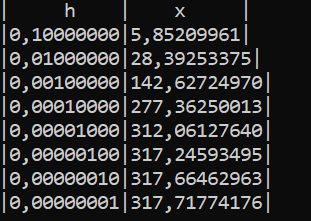
\includegraphics[scale=1]{img/question3_result.png}
  \caption{вывод программы}
  \label{fig:fig1}
\end{figure}

Результат: $u(2) = 317,717$

